

%\title{Fanning Friction Factors and Velocity Profiles for Turbulent, Incompressible Flow}


%\title{Fanning Friction Factors and Velocity Profiles for Turbulent, Incompressible Flow}
\documentclass{article}
\usepackage[english]{babel}
\usepackage[utf8]{inputenc}
\usepackage{johd}
\usepackage{dutchcal}

\title{Fanning Friction Factors and Velocity Profiles for Turbulent, Incompressible Flow}

\author{ Wesley Johanson, Chase Hartsell, Qiye Hu\\
        \small University Of California, Santa Barbara \\
        \small Chemical Engineering 180A Lab
        }

\date{April $13^{th}$, 2022}

\begin{document}

\maketitle


\noindent
\section*{Abstract}

Friction factors for turbulent water flow in a cylindrical pipe for different configurations, as well as the turbulent velocity profile, were determined for various flow rates. The aim of this is to compare frictional loss in straight tubes versus bends, and to see how the laminar sublayer region of the velocity profile gets smaller with increasing Reynold’s number. This was executed by measuring a pressure drop using transducers, and relating that pressure drop to the shear stress over the length of the tube to get the Fanning friction factor. These values were compared with empirical relations and the values and trends proved to be consistent. Having pipe bends should theoretically lead to more frictional loss, however not an appreciable difference was measured. To determine the velocity profile, a pitot tube was used to measure local velocity, and numerical integrations over the area were performed to compare our experimental flow rate results to the integrated flow rate values. The key results from this experiment were that friction factor decreases with increasing Re, although the pressure drop increases. The velocity profile of the fluid became flatter with increasing Re, and the spread of data also increased as expected due to more random turbulent fluctuations. 

\raggedright
\section*{Introduction}
Turbulent flow in a pipe, characterized by fluid flow with Reynolds number greater than 2100, causes frictional loss and a measurable pressure drop along for small diameter pipes.

\begin{equation} \label{eq:1}
\mathcal{Re} = \frac{D\langle V_{z} \rangle\rho}{\mu}
\end{equation}


The pressure drop can be related to the shear stress over the surface area of the viscous flow.\\

\begin{equation} \label{eq:2} 
2\pi\mathrm{RL}\tau_{0}=\pi\mathrm{R^2}\left(\rho_{0}-\rho_{l}\right) 
\end{equation}

\noindent \item \raggedright
The Fanning friction factor compares the shear stress on the fluid to its kinetic energy per volume.

\begin{equation} \label{eq:3} 
\tau_{0} =\left(\frac{1}{2} \rho\left< \nu_{z}\right>^2 \right)\mathcal{f} 
\end{equation}

\linebreak
\linebreak

\begin{equation} \label{eq:4} 
\mathcal{f} = \frac{\pi^2\mathrm{R}^5}{\rho\mathrm{Q}^2} \left( \frac{ \rho_{0} - \rho_{l}}{\mathrm{L}} \right)
\end{equation}

Friction factors decrease as flow becomes more turbulent, and the laminar sublayer region close to the wall shrinks while the velocity profile "flattens out." The objective of this experiment is to measure the friction factor of turbulent water flowing at various speeds and pipe configurations, and the velocity of the fluid throughout the diameter of the piping. The experimental data will be compared to empirical correlations for incompressible, turbulent flow.

\section*{Materials}
\begin{itemize}
    \item 55-gallon water tank
    \item 3/4 horsepower, 60 cycle, 220 volt, 3-phase electric motor with a variable speed drive
    \item Centrifugal pump (3450 rpm at 100\% power)
    \item 18" and 6" long, 1" diameter steel piping
    \item 0-5,0-10, and 0-25 psi pressure transducers
    \item 1" diameter pipe plugs and connectors
\end{itemize}

\begin{figure}[H]
\centering
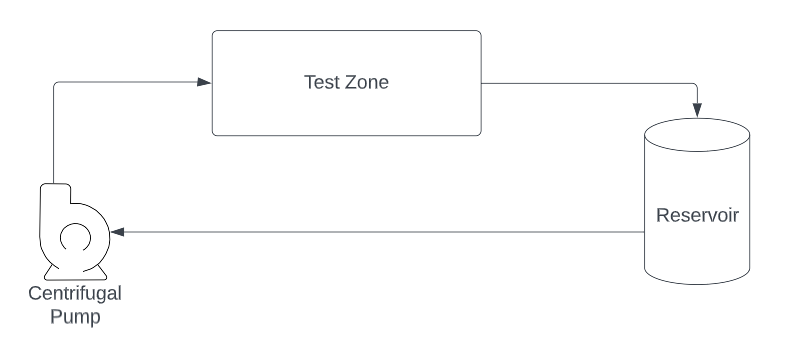
\includegraphics[width=0.8\textwidth]{images/Capture.PNG}
\caption{\label{fig1}Apparatus for measuring the Fanning friction factor of turbulent flow using pressure transducers. (Test zone varies with a straight 18" pipe, straight 6", a 12" 90 degree bend, a 16" 180 degree bend, and a 45" long pitot tube).}
\end{figure}

\section*{Experimental Methods}

 Flow rates were measured by diverting the water flow into a bucket, then the water was weighed and volumetric flow rate was determined by the ratio of water volume per unit time. The pressure drop was measured using pressure transducers, and a linear relation between current and pressure drop was observed and measured using regression (SEE APPENDIX A-). A pitot tube was used to measure the velocity profile and laminar sublayer region of the fluid flow. The local velocity of the fluid impacting the mouth of the tube is related to the pressure difference of the pitot tube (SEE APPENDIX B-).

\section*{Results}

As the flow rate increased, so did the pressure drop, however friction factor decreased. Having bends in the pipe increased frictional loss over the same length.  

\begin{figure}[H]
\centering
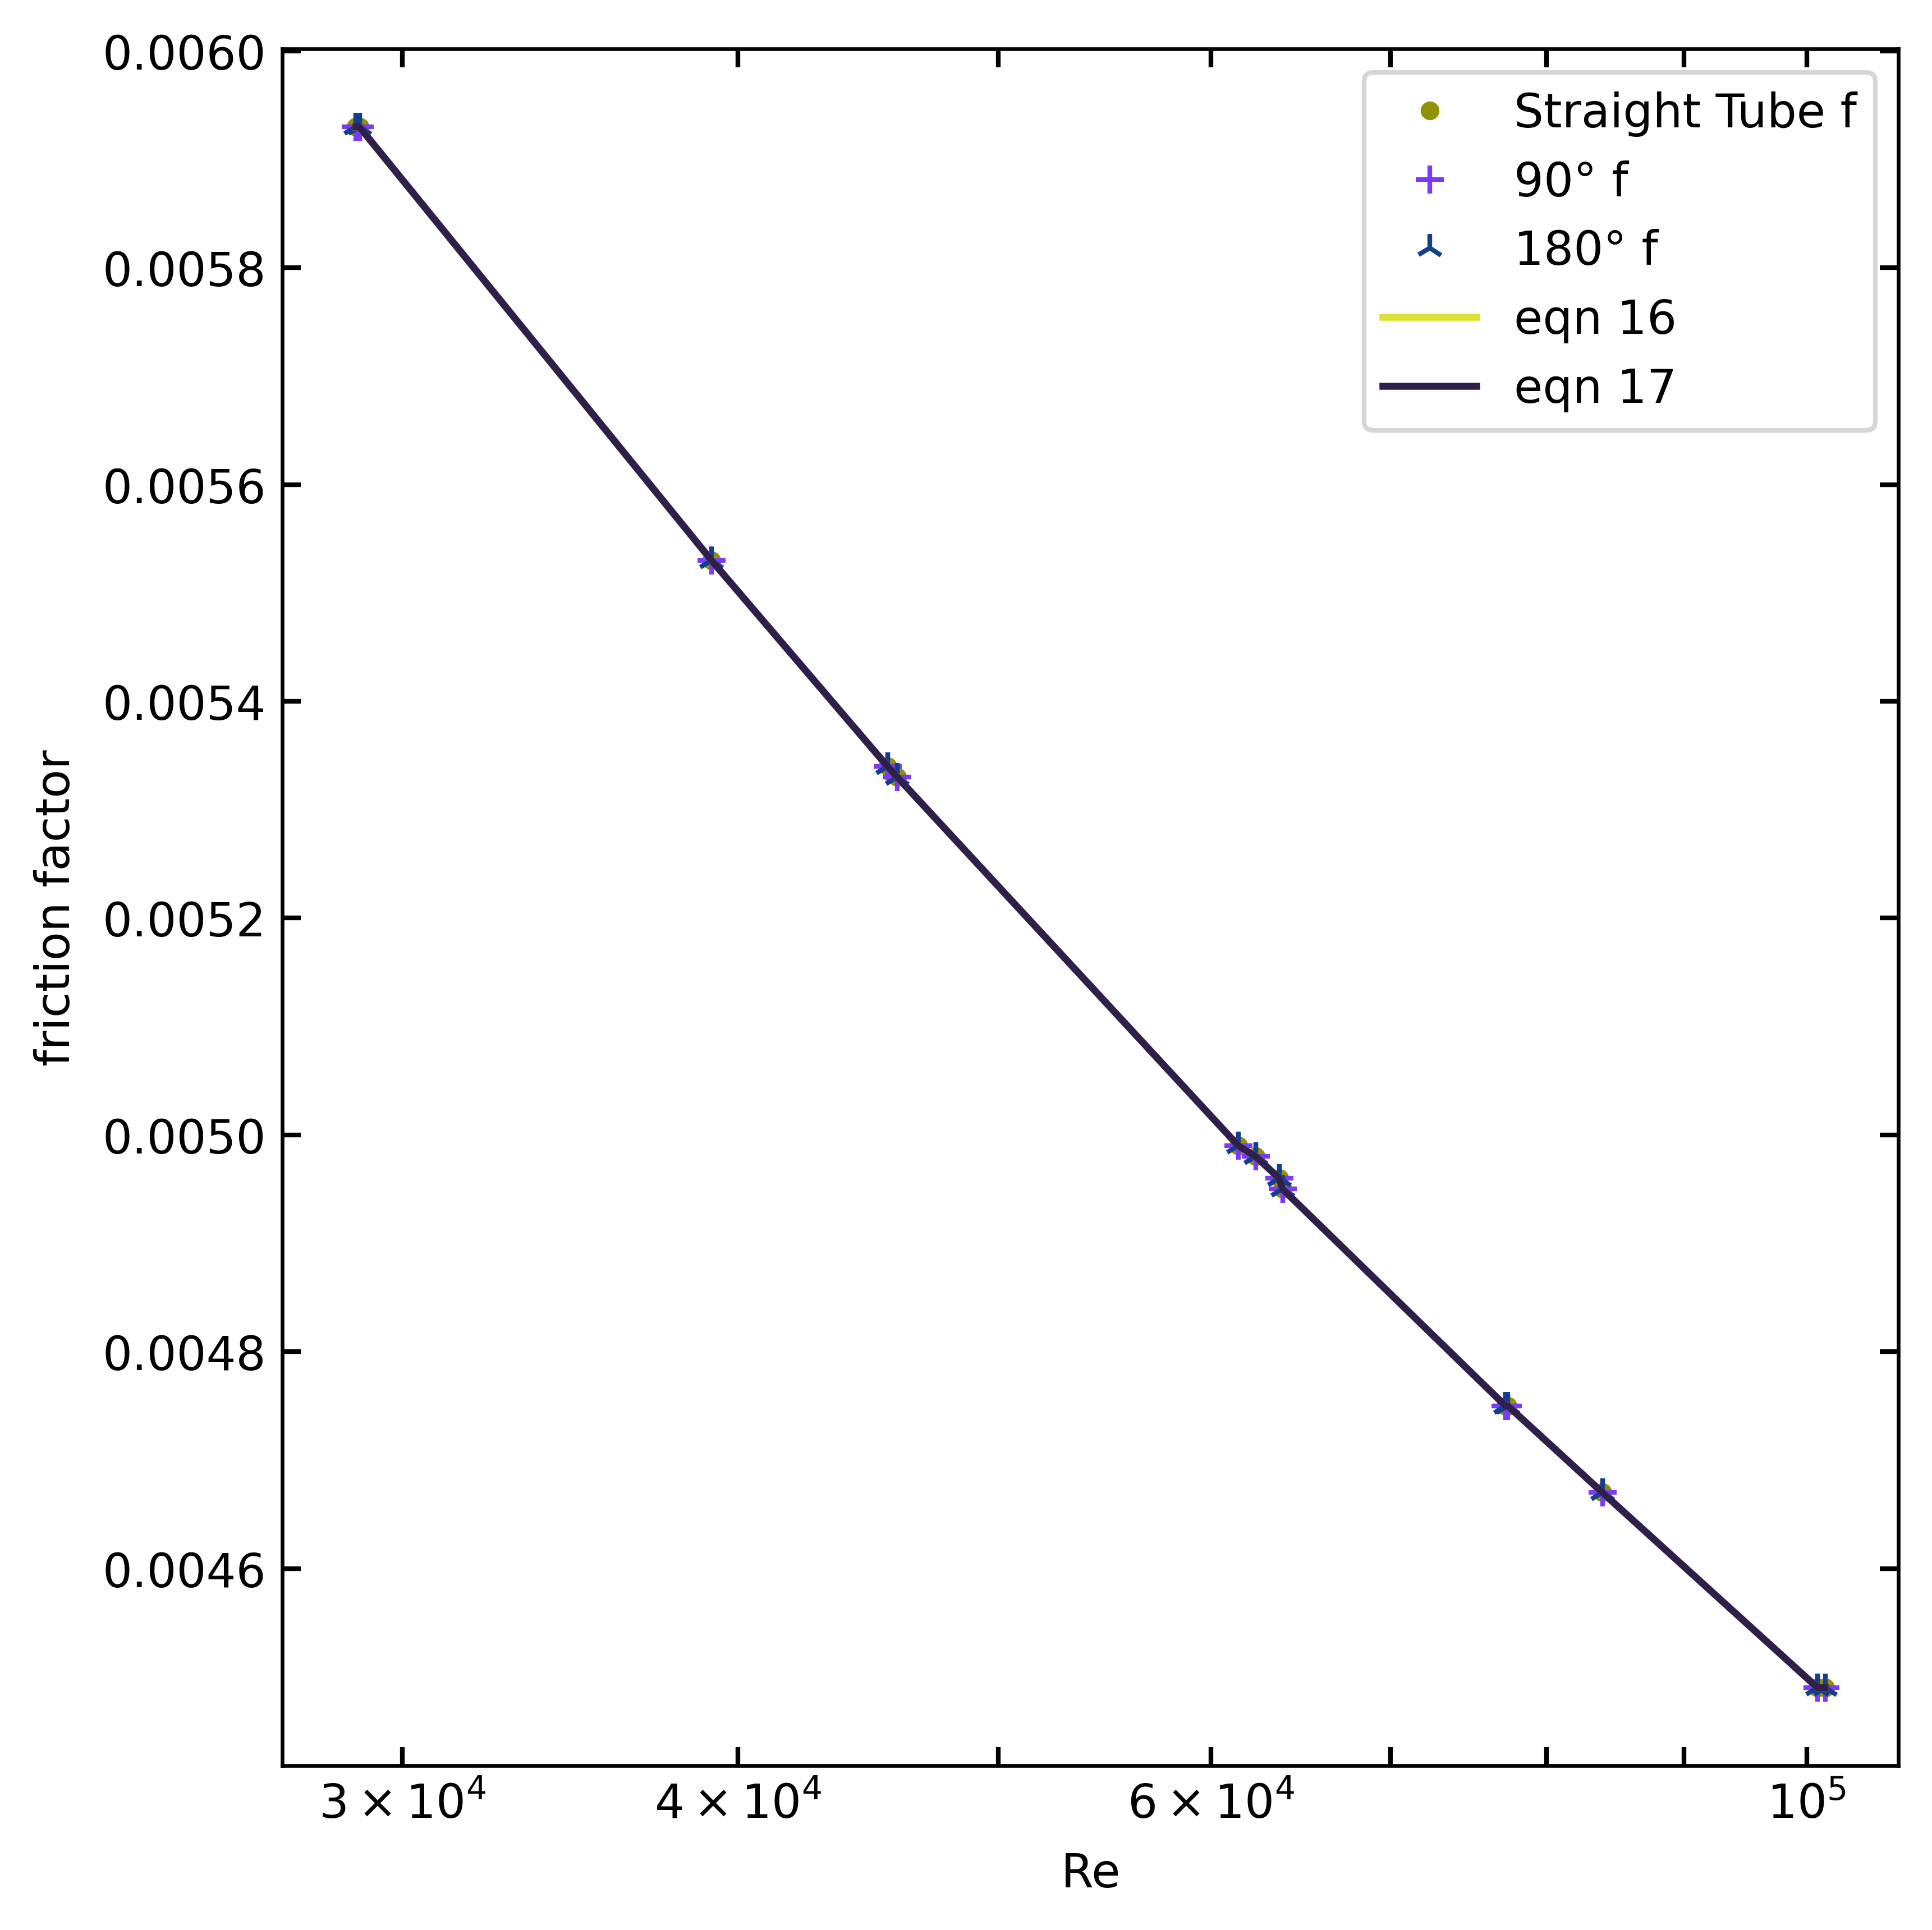
\includegraphics[width=0.6\textwidth]{images/1_plot.png}
\caption{\label{fig2}Fanning friction factors for turbulent, incompressible flow for different pump speeds and pipe configurations. The data is compared to empirical relations for turbulent flow.}
\end{figure}

The friction that each bend contributed to the pressure drop was consistent throughout each unique configuration.

\begin{figure}[H]
\centering
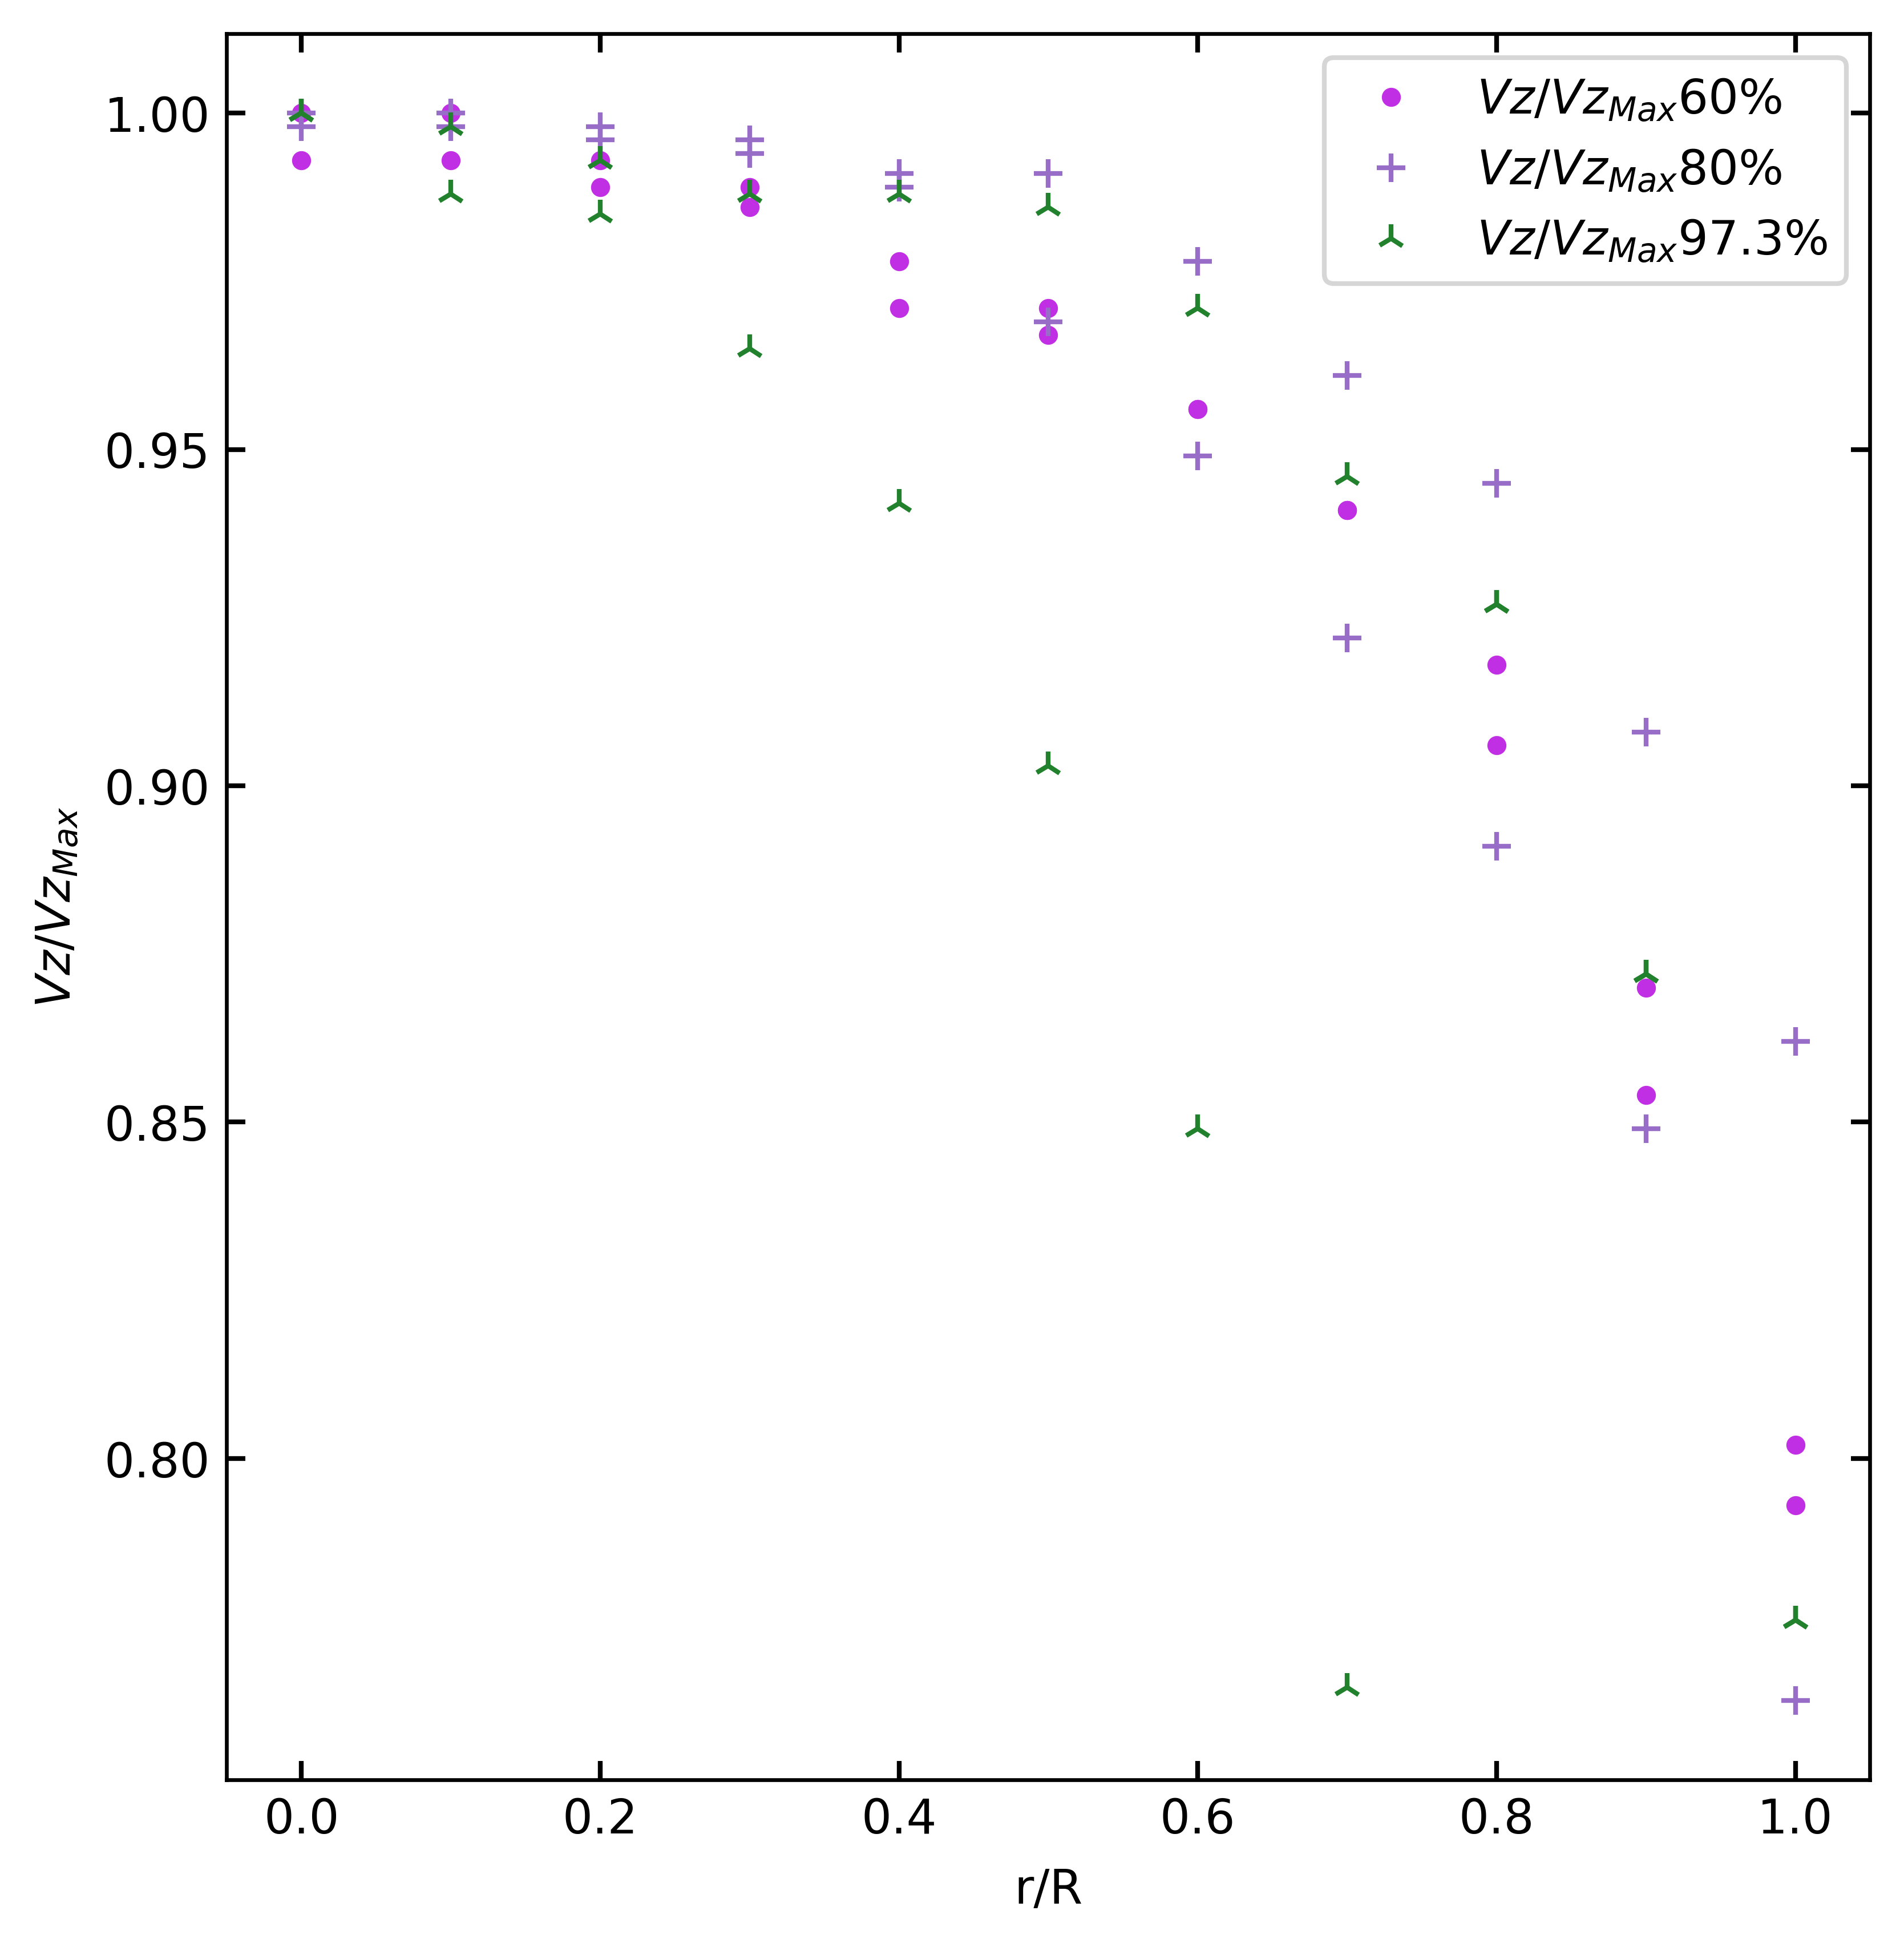
\includegraphics[width=0.6\textwidth]{images/0_plot.png}
\caption{\label{fig2}Dimensionless velocity profile for each pump speed. Spread of points at a given r/R value represent the spread in transducer readings and calculated velocity for each radius for two trials.}
\end{figure}

\begin{figure}[H]
\centering
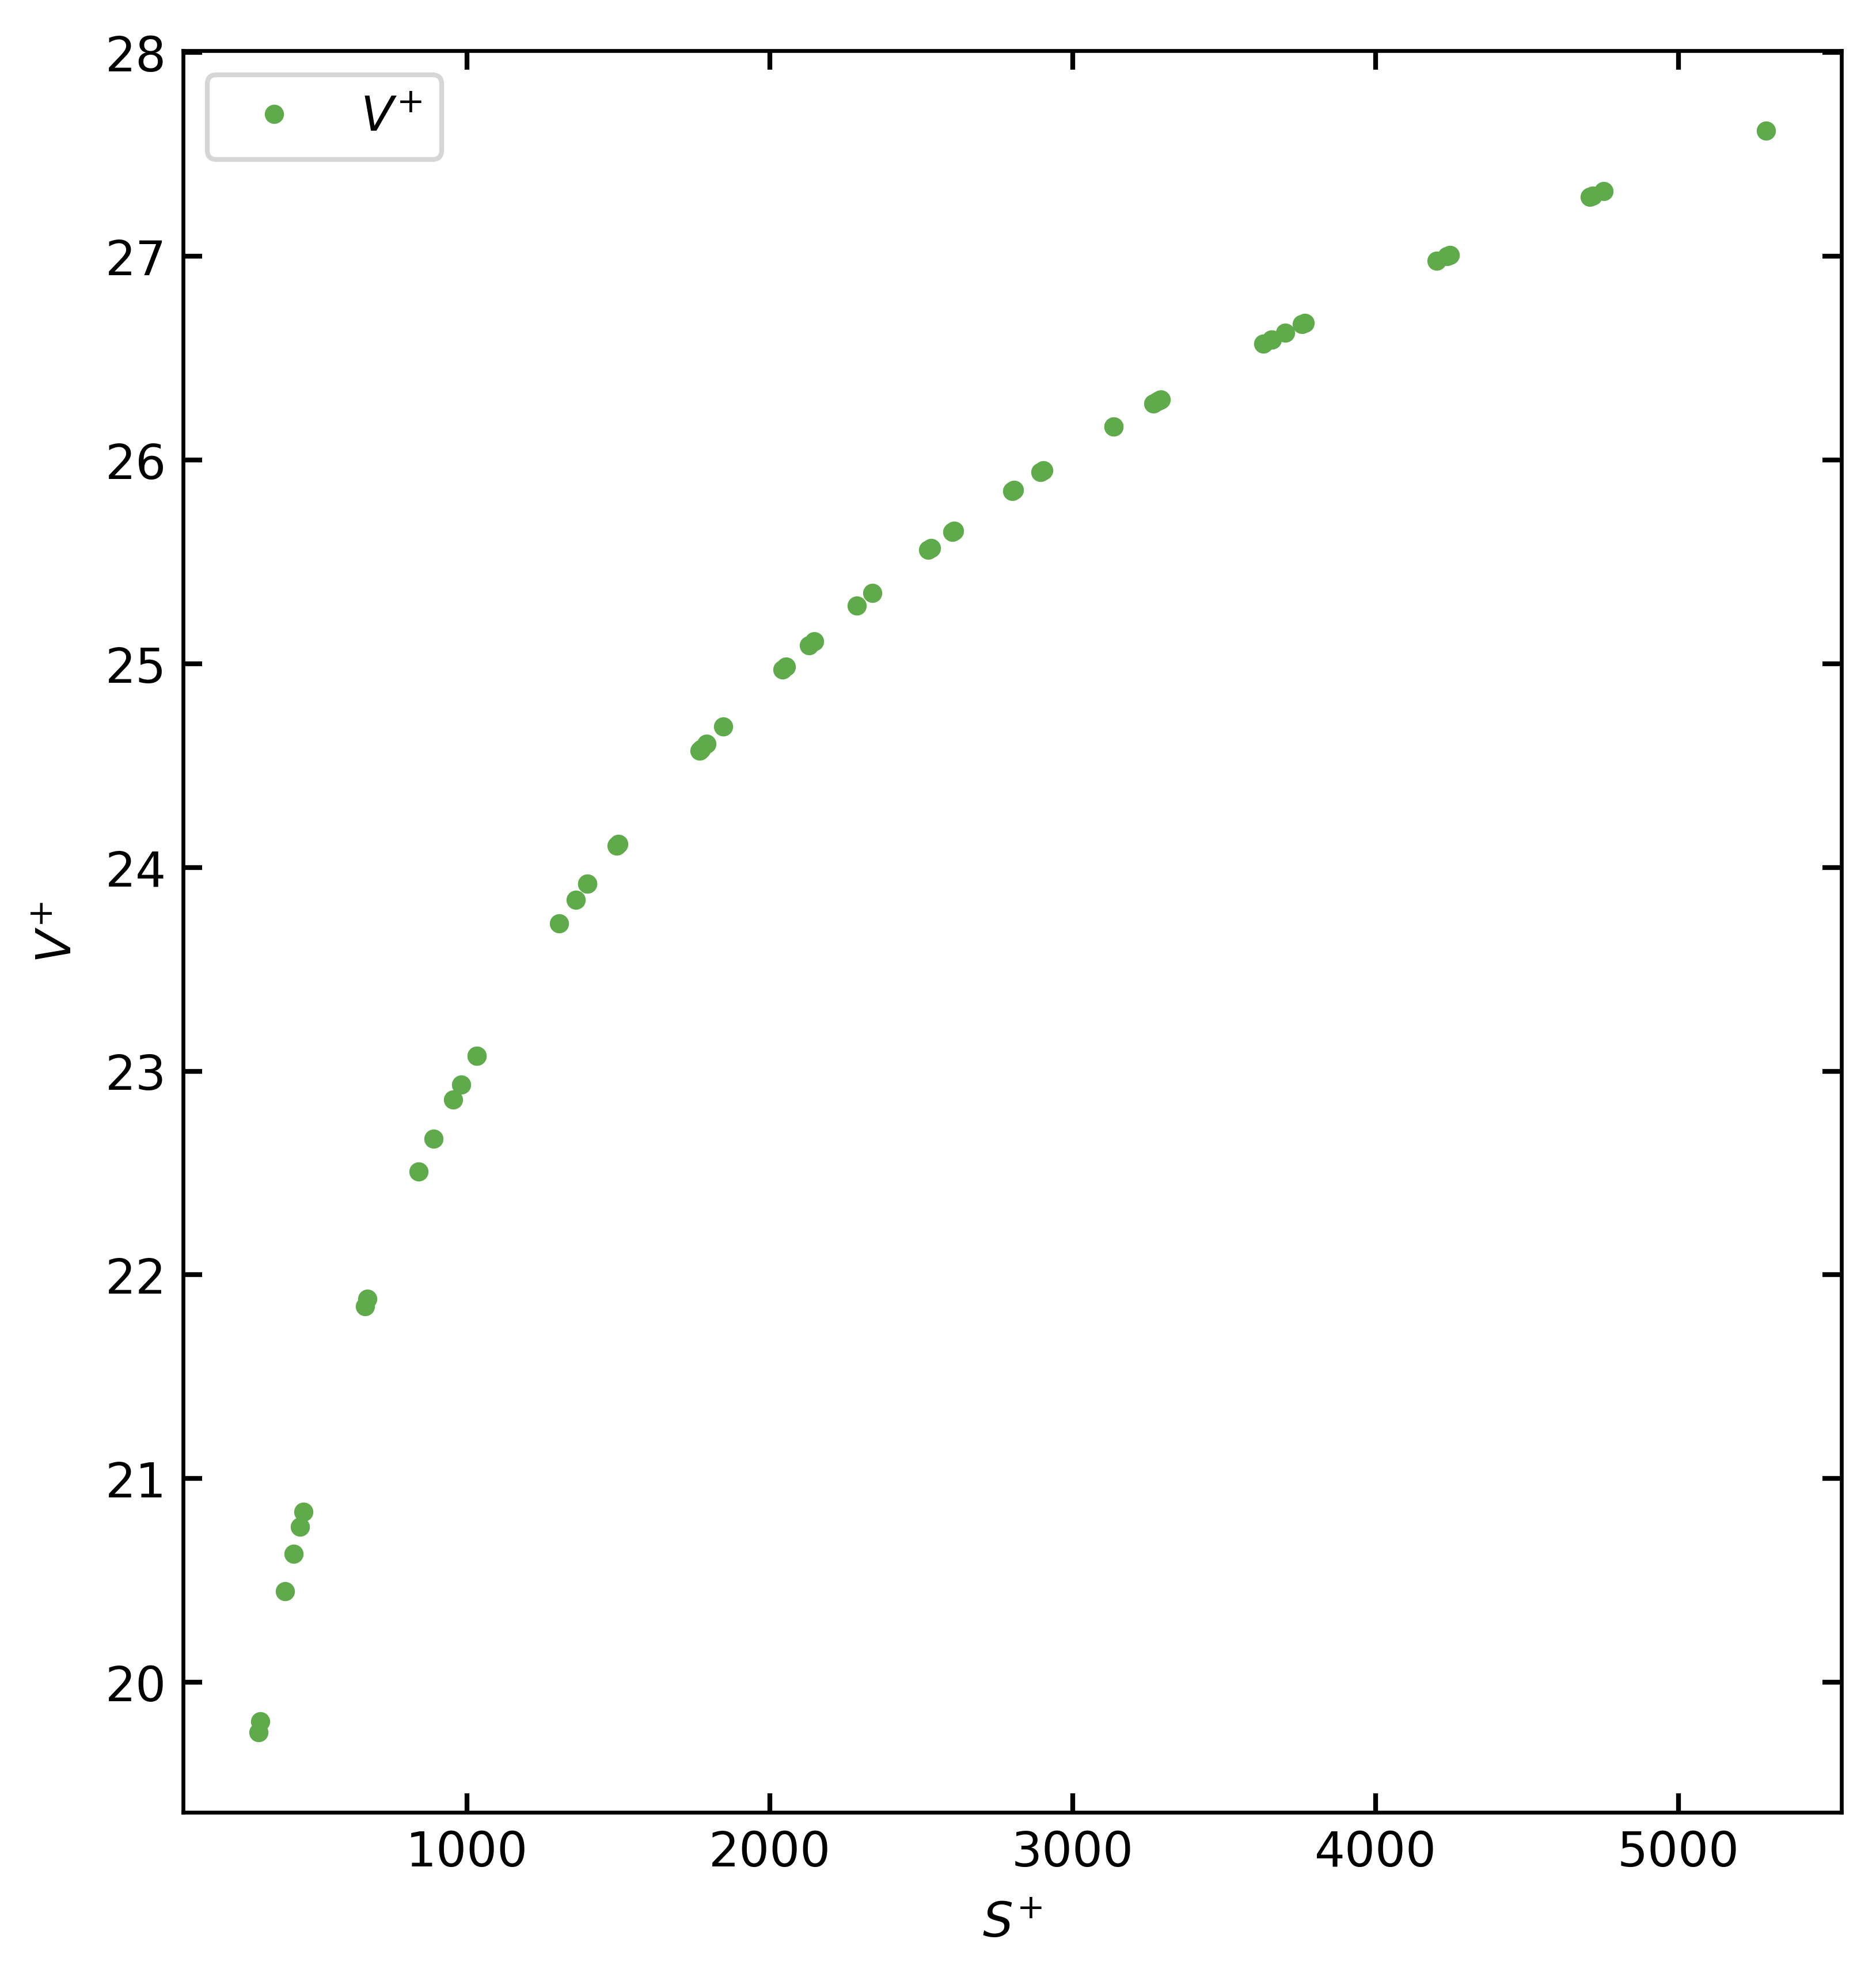
\includegraphics[width=0.6\textwidth]{images/2_plot.png}
\caption{\label{fig2} Universal velocity profile for turbulent fluid flow.}
\end{figure}

\section*{Discussion and Analysis}
Using Fanning’s friction factor and Newton’s Law of Viscosity, very similar friction factors were calculated when compared to the empirical relations (Appendix B) for each configuration of tubing.
\linebreak
\linebreak
They were consistent with the turbulent flow regime equations, and not consistent with the laminar regime equation. There were some discrepancies in the straight tube analysis, mainly for the 6" test section, but the bent tube data was extremely consistent. The reason that the 6" inch test section had such a higher reported friction factor could be because the pressure drop from the transducer inlets and T-plugs plays a much bigger role when looking at shorter sections. Estimating the flow rates was also not very precise, as the timer was human controlled, so this could have caused inconsistencies in the calculated Reynold's Number. The propagated error for each friction factor turned was +/- .0004, which would make the two inconsistent data points fit closer with our model. The empirical relations showed very similar trends in the friction factor, however they are all slightly lower than what we expected. This could also be due to added pressure drop from the transducer inlets and plugs. Adjusting the "minus 0.4"  equation (9) in Appendix B to .2 causes a shift in the friction factors that bring them closer to our experimental data. \linebreak
\linebreak

For the test sections with bends in the pipe, not a very significant increase in friction factor was observed as expected. Literature values state that depending on the radius of the bend/diameter of the pipe, the frictional loss factor of having a bend could cause a 120-180\% increase in frictional loss, however very similar, if not lower, friction factors were observed compared to the straight tube. This would lead us to say that given a shorter straight tube, we would observe the same frictional loss, however this is known to not be true. However, for each configuration we saw an overall consistent pressure drop. It is worth noting that the pressure drop effect from valves were going to be measure as well but apparatus limitations restricted us from measuring the pressure drop, as it was too high. The fact that we observed the T-plugs reducing the pressure proves that a valve would also have an effect, even more so than the bends.
\linebreak
\linebreak
The velocity profiles of the fluid (Figure 3.) at each pump speed showed that more turbulent flow has a higher spread in velocity. Due to the apparatus only allowing us to go up half way up the tube, a full velocity profile was not able to be produced over the whole diameter. The laminar sublayer did appear to get smaller as flow became more turbulent, however the greater spread in data does make it hard to get a quantitative measurement for how different the sublayer is. This spread was determined by comparing two trials of a given flow rate. As expected, the velocity profile did flatten out more as flow became more turbulent. This is because the randomly directed eddies average out to have a pretty constant velocity throughout the diameter over time. The universal velocity profile in Figure 4. is an interesting way of non-dimensionalizing the system. An implication of this approach is that it does not recognize the center of the tube where the velocity profile should be flat, so this data is not as helpful for distances far from the pipe wall. The main take away from this is that there is obviously a lot of viscous interactions close to the wall that give it a laminar sublayer region. 



\section*{Conclusions}

The Fanning friction factors that were experimentally determined were very close and followed the same trends as the empirical relations. A greater spread in data was observed for more turbulent flow rates, as expected. Pressure drop from the inlet and outlet plugs proved to have more of an affect than we thought, and the data for the 6" inch tube was not as consistent as all of the other values, so it is worth noting that end effects in the pipe do make an appreciable difference in frictional loss. \linebreak
\linebreakhttps://www.overleaf.com/project/625c6995f63258a623a07335
The velocity profiles looked as expected, and the laminar sublayer regions did get smaller for more turbulent flow. Random fluctuations in transducer readings did make it hard to get an accurate time-averaged value for each transducer reading, however the trends were still what we expected despite the spread of data. 

\section*{References}

Bird, R.B., W.E. Stewart, and E.N. Lightfoot, Transport Phenomena, John Wiley and Sons, New York (1960).
\linebreak
\linebreak 
Department of Aerospace Engineering | Department of ... http://ae.sharif.edu/~viscousflow/Schlichting%20-%20Boundary%20Layer%20Theory.pdf. 
\linebreak
\linebreak

McCabe, W.L., J.C. Smith, and P. Harriott, Unit Operations of Chemical Engineering, Fifth Edition, McGraw-Hill, Inc., New York (1993).
\linebreak
\linebreak 
“Friction Losses in Pipe Fittings.” Metro Pumps, April 17,2022. https://www.metropumps.com/ResourcesFrictionLossData.pdf. 
\linebreak 
\linebreak 
Kudela, Henryk. "Turbulent Flow." Faculty of Mechanical and Power Engineering. Wroclaw University of Science and Technology. Lecture.   
\linebreak
\linebreak
Schlichting H., Kestin,J., Boundary-Layer Theory, SeventhEdition, McGraw-Hill, Inc., New York (1979).  

\centering \section*{Appendix A: Raw Data} \raggedright
\begin{itemize}
\item Experiments were performed in the 40-97.3\% pump speed range, as pump efficiency was not great at low speeds.
\item The pressure drop was measured using a pressure transducer, and a linear relationship between current and pressure drop was observed and measured using regression (calibration data 3.92mA = 0psi, 25mA = 20psi).
\end{itemize}

\begin{figure}[H]
\centering
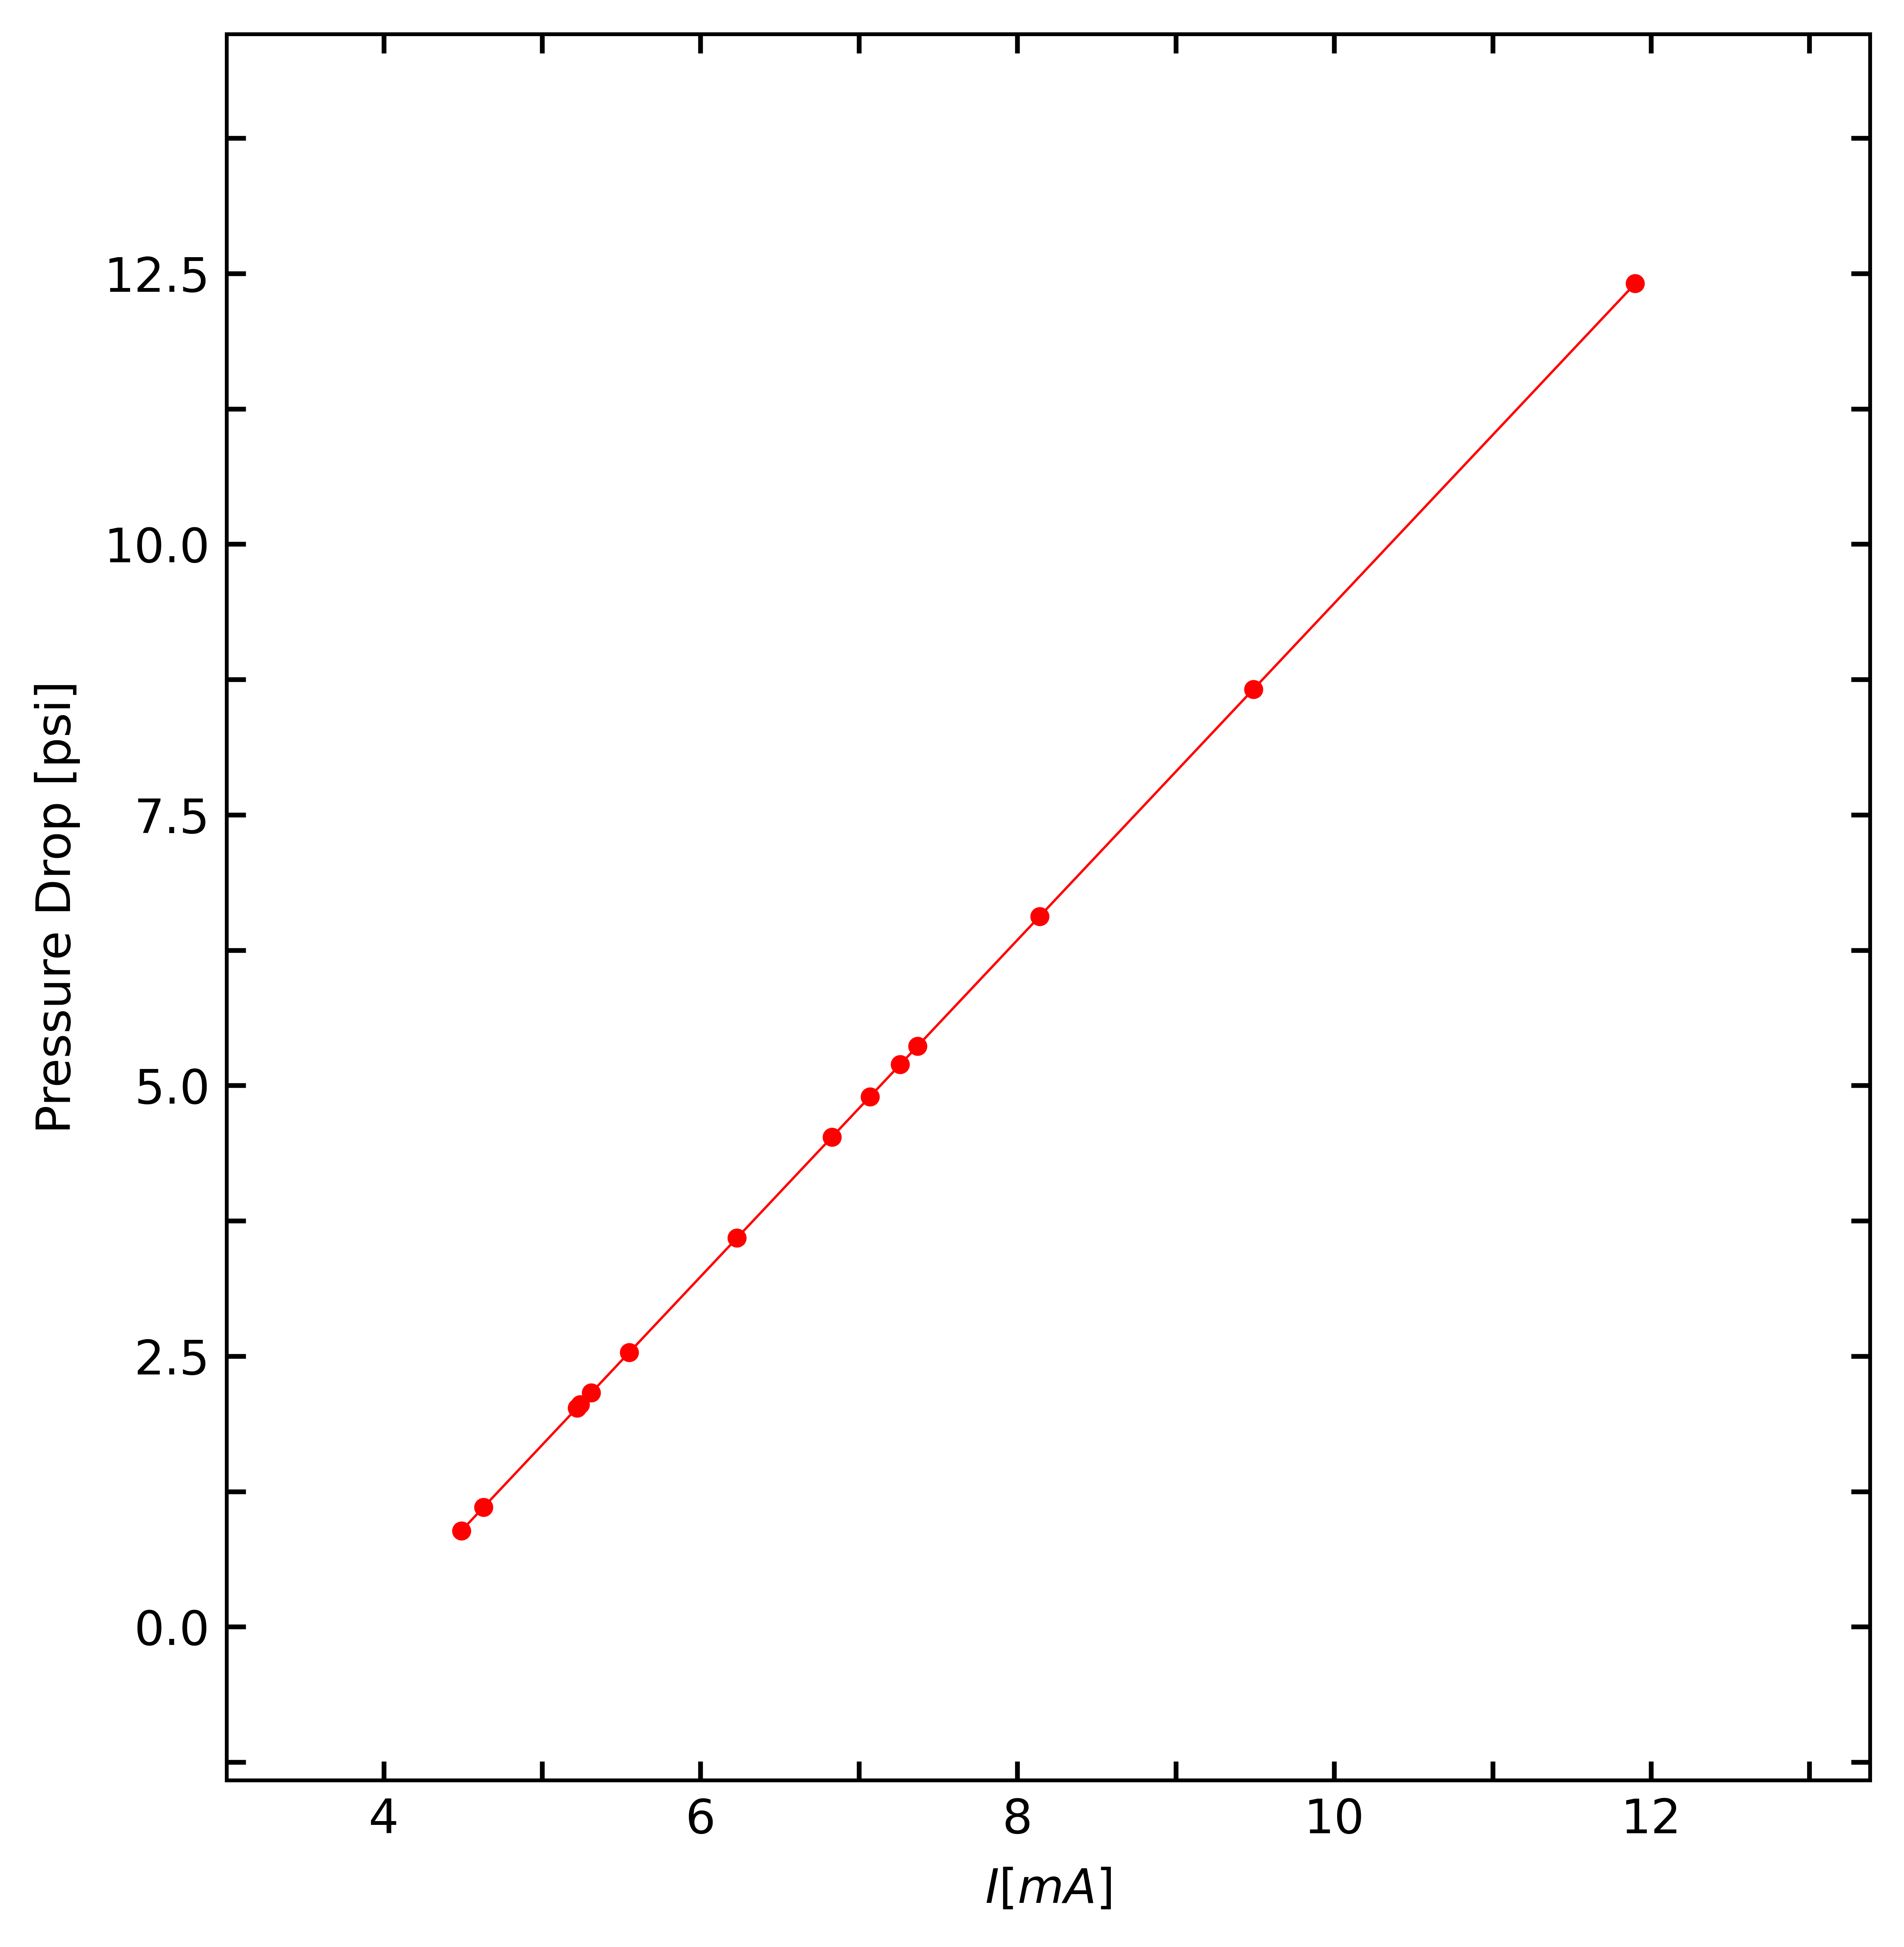
\includegraphics[width=0.8\textwidth]{images/transducer_psi_mA.png}
\caption{\label{fig1}Calibration to find the linear relationship between the current reading of a 25mA pressure transducer and the associated pressure drop across the tube. A reading of 3.92 mA corresponds to a 0 psi drop and 20mA shows the maximum reading of a 25 psi drop.}
\end{figure}

\caption{\label{fig1}\\ Table 1: Different Friction Factor Models are valid within different ranges of the Reynolds's number}
\linebreak \\ 
\centering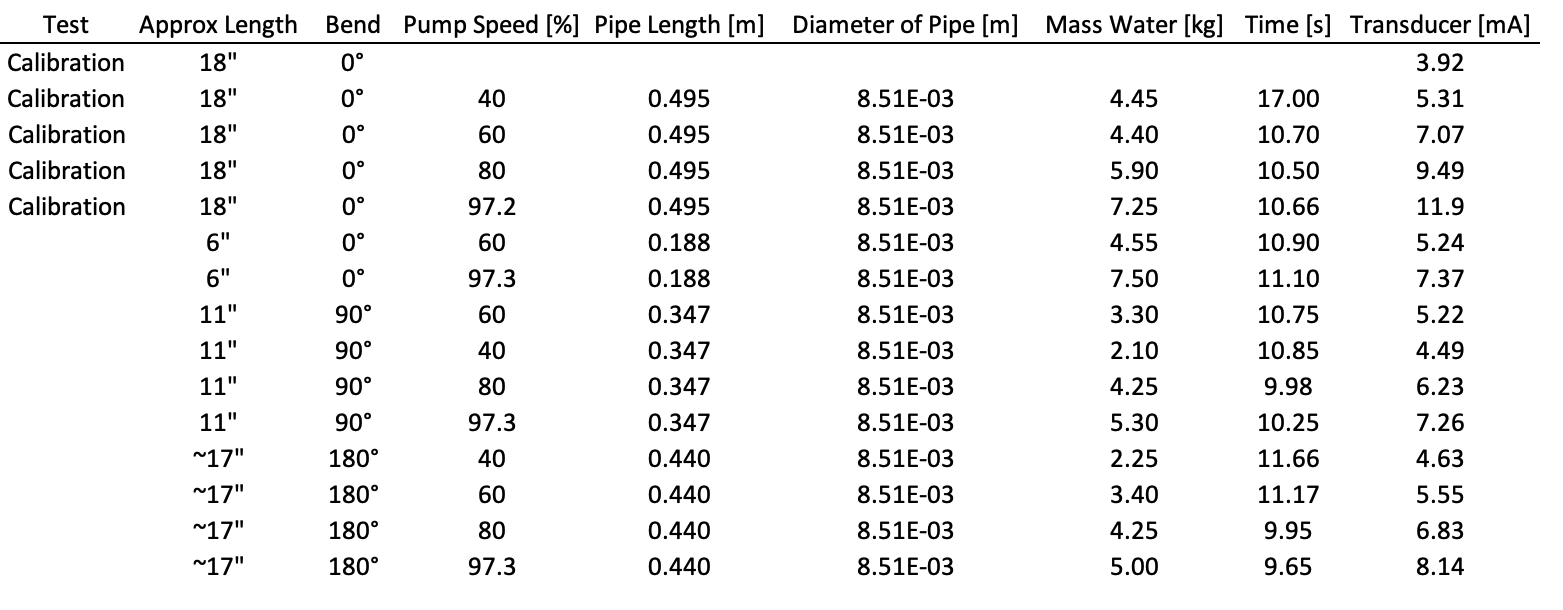
\includegraphics[width=1\textwidth]{images/rawdata.png}\raggedright


\caption{\label{fig1}\\ Table 2: Calculating the dimensionless velocity with respect to the dimensionless distance from the wall to obtain a universal velocity profile for Figure 4.}
\linebreak \\ 
\centering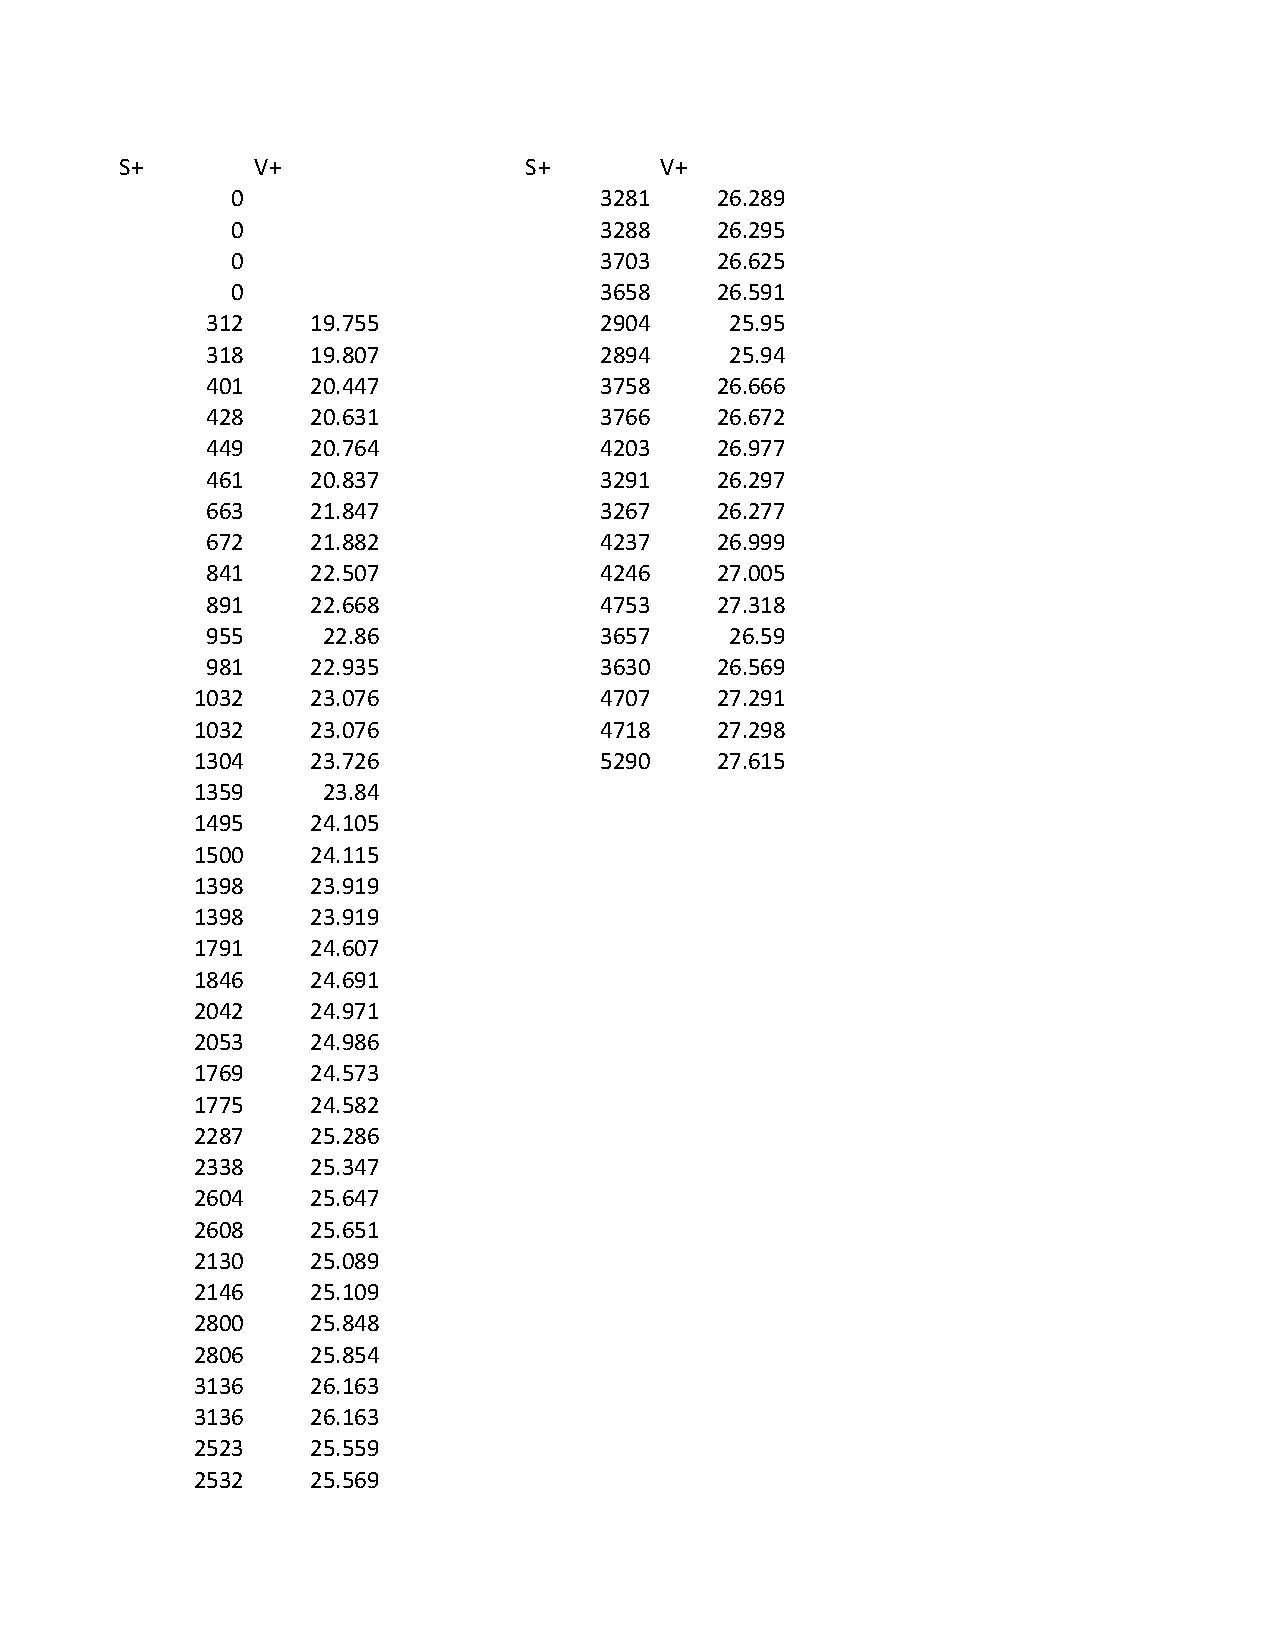
\includegraphics[width=0.8\textwidth]{images/table_2.pdf}\raggedright

\caption{\label{fig1}\\ Table 3: Data for each Fanning friction factor for each configuration with its respective comparison to empirical relations.}
\linebreak \\ 
\centering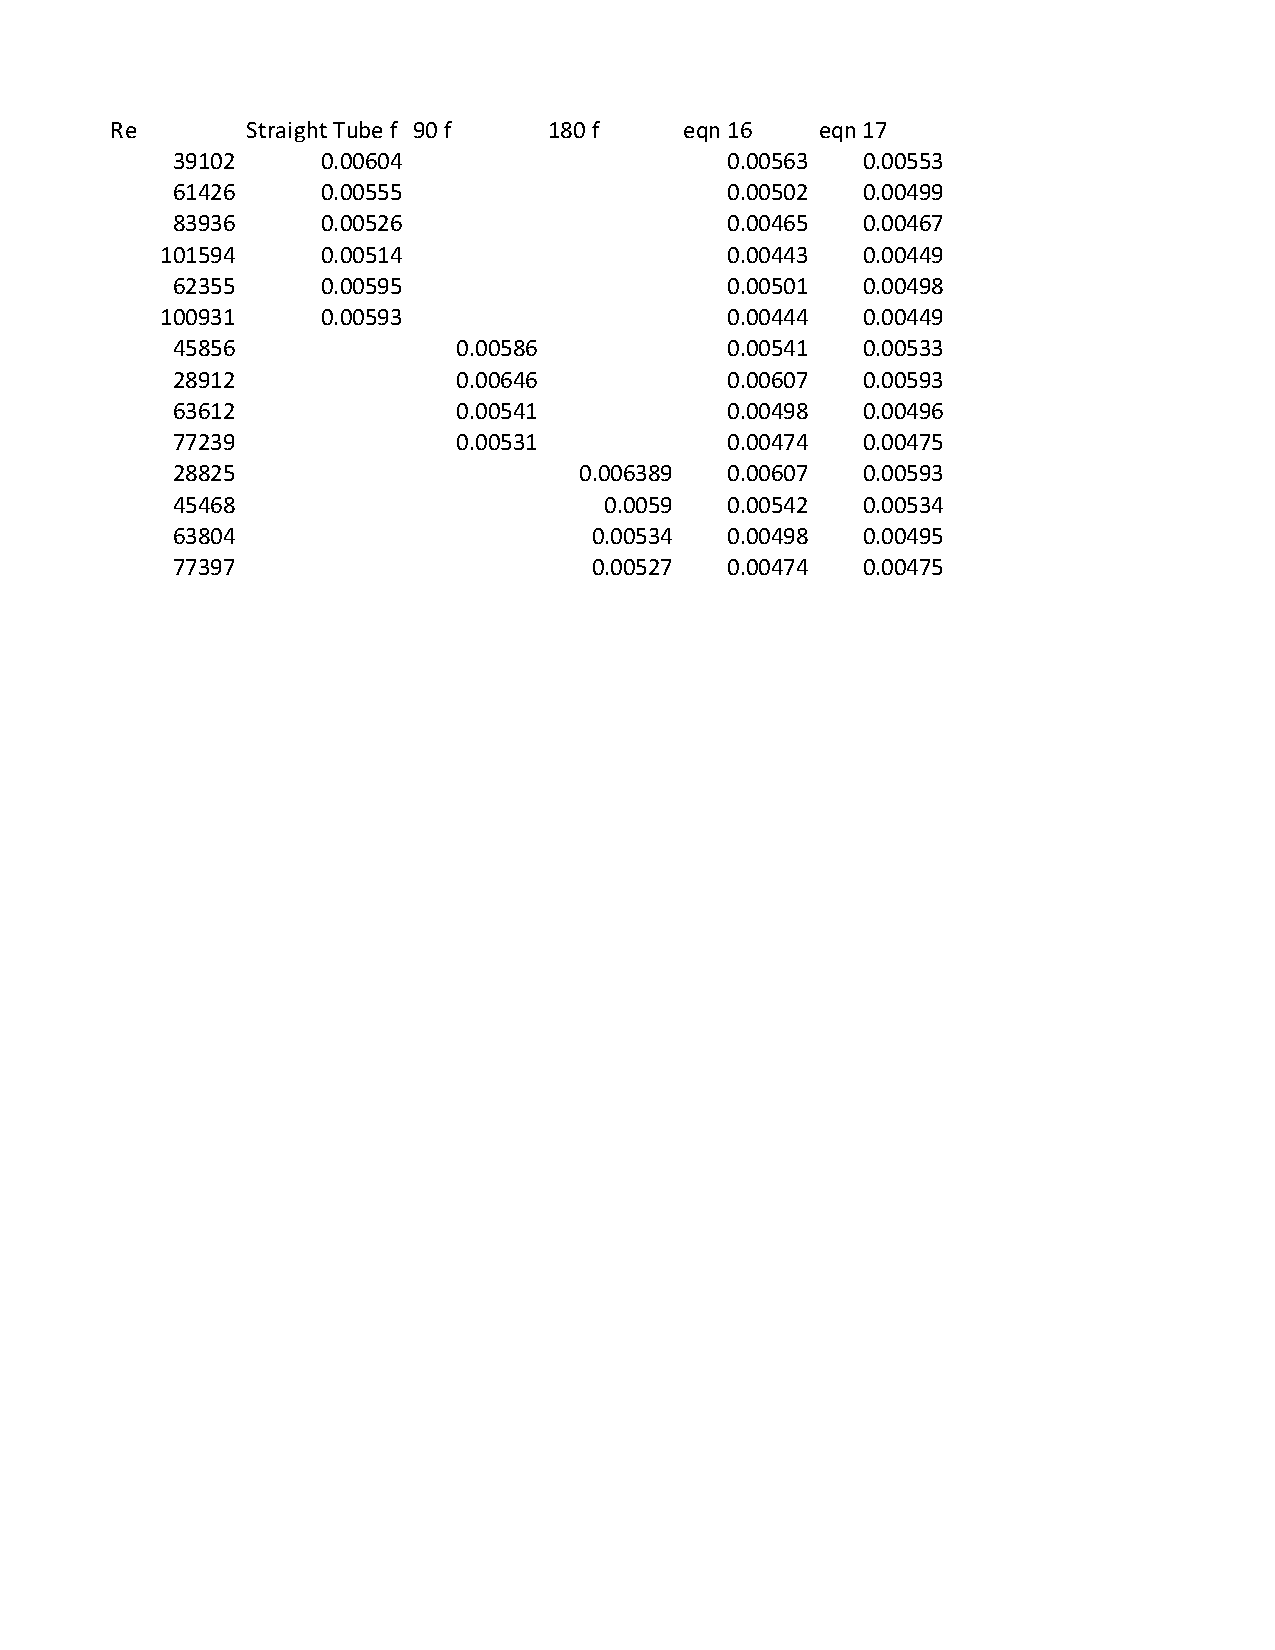
\includegraphics[width=0.8\textwidth]{images/table_1.pdf}\raggedright

\caption{\label{fig1}\\ Table 4: Local velocity compared to maximum velocity. These are plotted on Figure 3 to see how increasing Reynold's number affects the length of the laminar sublayer region.}
\linebreak \\ 
\centering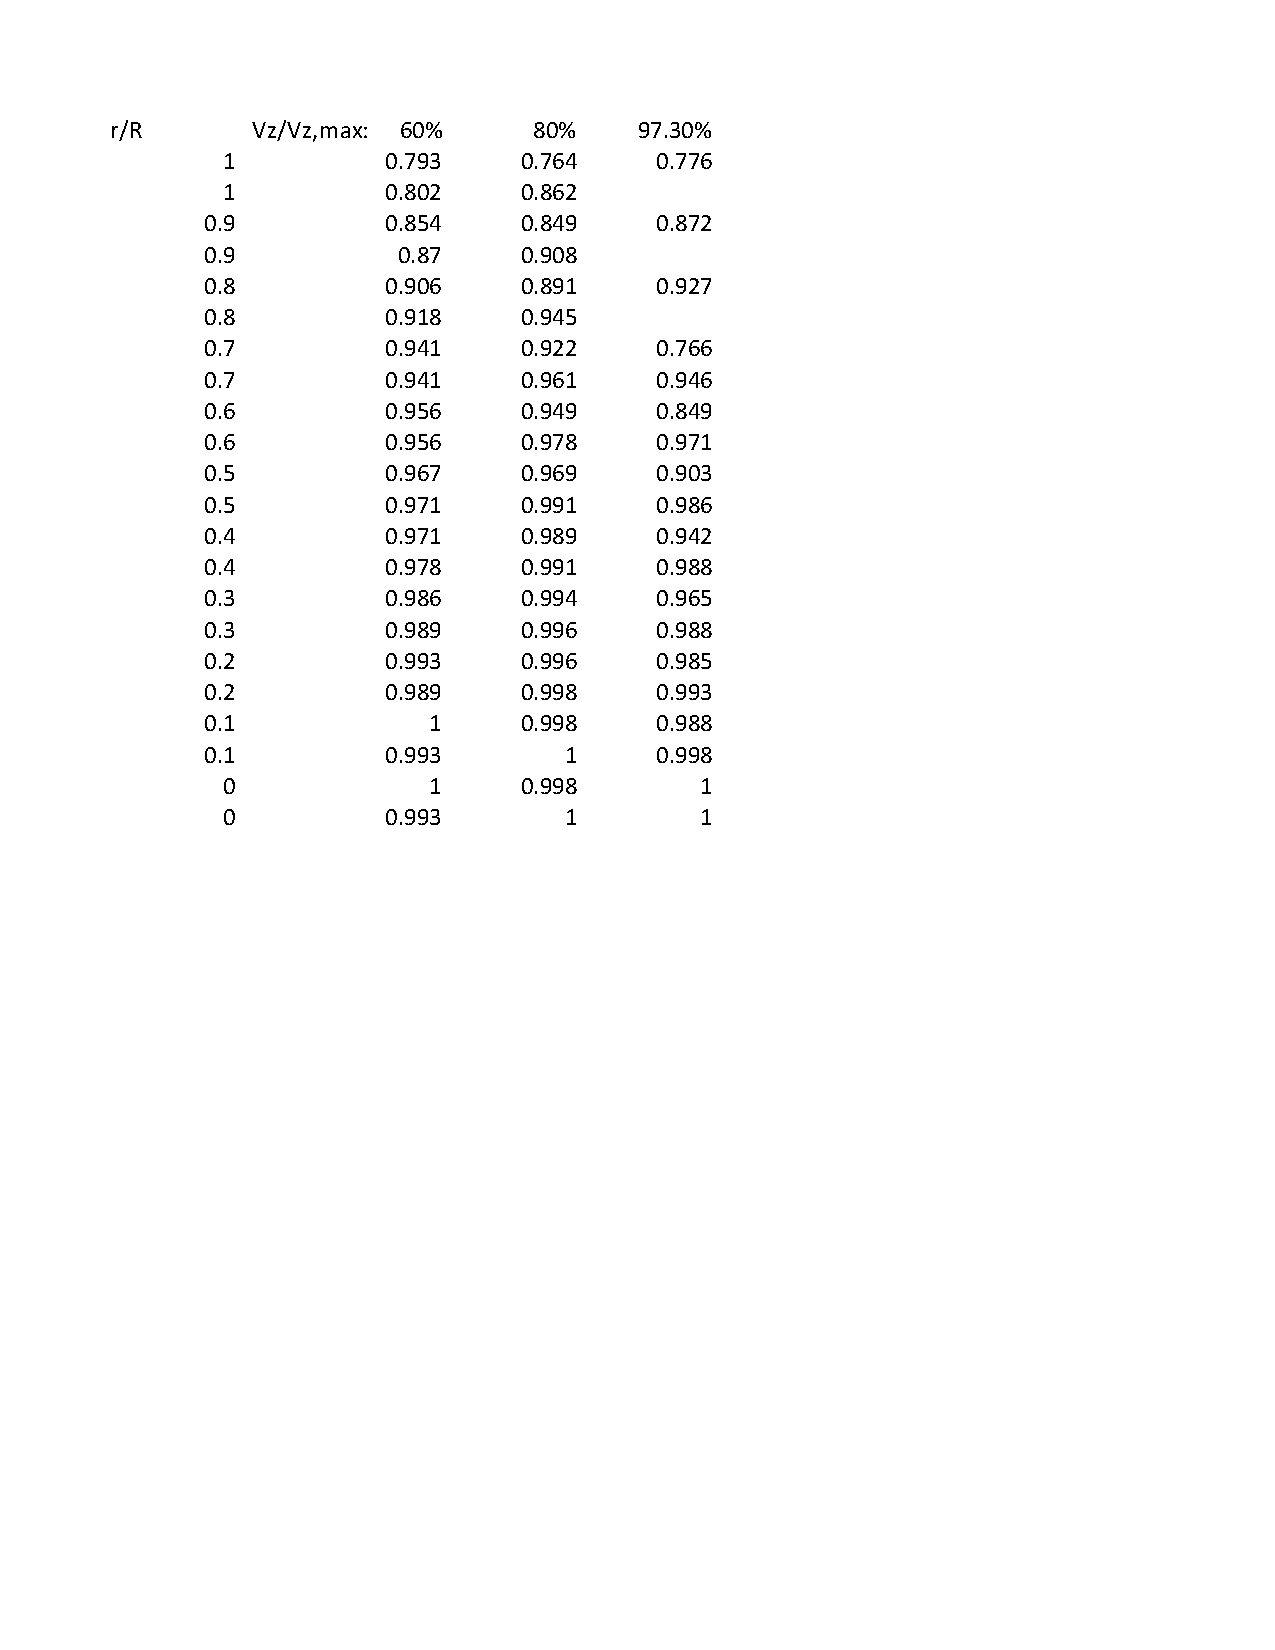
\includegraphics[width=0.8\textwidth]{images/table_0.pdf}\raggedright


\centering \section*{Appendix B: Sample Calculations} \raggedright

\begin{equation} 
Q=\frac{Volume}{time}
\end{equation}
These are the empirical equations relating friction factor to Re. Equation 6 is valid for laminar flow and equations 7, 8, and 9 are valid for turbulent flow.

\begin{equation} 
\mathcal{f}=\frac{16}{\mathcal{Re}}
\end{equation}


\begin{equation} 
\mathcal{f} = \frac{0.0791}{\mathcal{Re}^{1/4}}
\end{equation}


\begin{equation} 
\mathcal{f} = \frac{0.0791}{\mathcal{Re}^{1/4}}
\end{equation}

\begin{equation} 
\frac{1}{\mathcal{\sqrt{f}}} = 4.0Log_{10}(\mathcal{Re}\sqrt{f})-0.40
\end{equation}

The universal velocity profile was calculated for values of s+ above 26 using:

\begin{equation} \label{eq:10}
\mathcal{v^{+}} = \frac{1}{0.36}ln(\mathcal{s^{+}})+3.8  \quad\quad \emph{for} \quad\quad \mathcal{s^{+}\ge26}
 \end{equation}

Error propagation: The scale used was only accurate to the .05 kg, which created uncertainty in the flow rates measurements that carried through to the Reynold's number calculations. Also the stop watch timing was estimated to have an uncertainty of about 1/4 of a second, which also carried through the flow rate and Re calculations.

\centering \section*{Appendix C: Program Files} \raggedright



\end{document}